\chapter{ユーザインターフェース}
\section{画面遷移}
\begin{figure}[H]
    \centering
    \begin{minipage}[b]{.45\textwidth}
        \centering
        \begin{framed}
            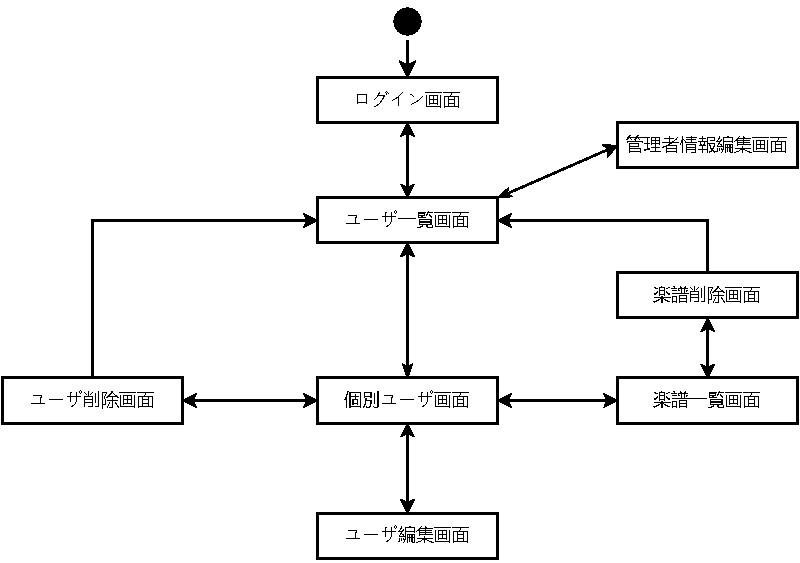
\includegraphics[keepaspectratio,width=\textwidth]{ui/管理者側画面遷移図.pdf}
        \end{framed}
        \caption{管理者側画面遷移図}
    \end{minipage}
    \begin{minipage}[b]{.45\textwidth}
        \centering
        \begin{framed}
            \vspace{.2cm}
            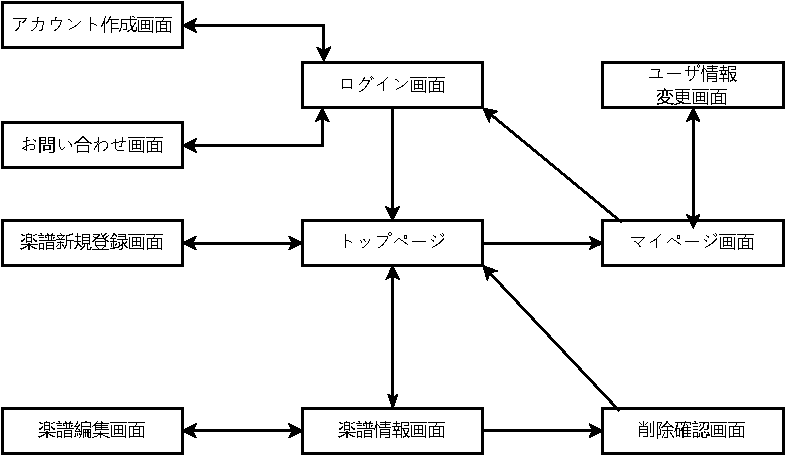
\includegraphics[keepaspectratio,width=\textwidth]{ui/利用者側画面遷移図.pdf}
        \end{framed}
        \caption{管理者側画面遷移図}
    \end{minipage}
\end{figure}
\section{UI View}
\subsection*{ユーザ側UI(→p.\pageref{fig:ui-view:user})}
\subsection*{管理者側UI(→p.\pageref{fig:ui-view:admin})}
「ログイン」は,ユーザ側UIと共通のため,p.\pageref{fig:ui-view:user}に記載している.
\begin{figure}[p]
    \newcommand{\vuser}[2]{\begin{minipage}[b]{.32\textwidth}\centering\includegraphics[keepaspectratio,width=\textwidth]{ui/user/#1.png}\caption{#2}\end{minipage}}
    \centering\label{fig:ui-view:user}
    \vuser{0-ログイン}{ログイン}
    \vuser{1-利用登録}{利用登録}
    \vuser{2-トップページ画面}{トップページ}\\
    \vuser{3-楽曲登録:編集}{楽譜登録,編集}
    \vuser{4-マイページ}{マイページ}
    \vuser{10-楽曲操作決定}{楽譜詳細画面}\\
    \vuser{5-楽曲編集確認}{楽曲編集}
    \vuser{7-ユーザパスワード変更}{パスワード変更}
    \vuser{7-ユーザ情報編集}{ユーザ情報編集}\\
    \vuser{7-ユーザ情報編集エラー}{ユーザ情報編集エラー}
    \vuser{8-ユーザ情報削除確認}{ユーザ情報削除確認}
    \vuser{9-お問い合わせ}{お問合せ画面}
\end{figure}
\begin{figure}[p]
    \newcommand{\vadmin}[2]{\begin{minipage}[b]{.32\textwidth}\centering\includegraphics[keepaspectratio,width=\textwidth]{ui/admin/#1.png}\caption{#2}\end{minipage}}
    \centering
    \label{fig:ui-view:admin}
    \vadmin{0-トップページ}{トップページ}
    \vadmin{1-操作選択}{操作選択}
    \vadmin{2-ユーザ情報編集}{ユーザ情報編集}\\
    \vadmin{2-ユーザ情報編集エラー}{ユーザ情報編集エラー}
    \vadmin{2-ユーザ情報編集確認}{ユーザ情報編集確認}
    \vadmin{3-ユーザ削除確認}{ユーザ削除確認}\\
    \vadmin{4-ユーザ楽曲DB}{楽譜DB一覧}
    \vadmin{4-ユーザ楽曲削除確認}{楽譜削除確認}
    \vadmin{5-管理者情報編集}{管理者情報編集}
\end{figure}